\documentclass[aspectratio=169]{beamer}

\usetheme{Boadilla}
\usefonttheme{professionalfonts}
\setbeamertemplate{navigation symbols}{}
\setbeamertemplate{itemize items}[circle]
\setbeamertemplate{enumerate items}[default]
\setbeamertemplate{headline}{}

\usepackage[utf8]{inputenc}
\usepackage[T1]{fontenc}
\usepackage{lmodern}
\usepackage{amsmath}
\usepackage{booktabs}
\usepackage{tabularx}
\usepackage{array}
\usepackage{hyperref}
\usepackage[strings]{underscore}
\usepackage{listings}
\usepackage{tikz}
\usetikzlibrary{arrows.meta,positioning,fit,calc,shapes.geometric}
\usepackage{xcolor}

\definecolor{courseblue}{HTML}{12355B}
\definecolor{coursegold}{HTML}{C98A2E}
\definecolor{courseice}{HTML}{EEF3F8}
\definecolor{coursegreen}{HTML}{2F6B4F}
\definecolor{coursegray}{HTML}{4B5563}
\definecolor{codebg}{HTML}{F7F9FC}
\definecolor{codecomment}{HTML}{5E6C84}
\definecolor{codestring}{HTML}{0B6E4F}

\setbeamercolor{palette primary}{bg=courseblue,fg=white}
\setbeamercolor{palette secondary}{bg=coursegold,fg=white}
\setbeamercolor{palette tertiary}{bg=courseblue,fg=white}
\setbeamercolor{palette quaternary}{bg=coursegold,fg=white}
\setbeamercolor{structure}{fg=courseblue}
\setbeamercolor{frametitle}{bg=courseice,fg=courseblue}
\setbeamercolor{title}{fg=courseblue}
\setbeamercolor{block title}{bg=courseblue,fg=white}
\setbeamercolor{block body}{bg=courseice,fg=black}
\setbeamercolor{normal text}{fg=black,bg=white}
\setbeamercolor{alerted text}{fg=coursegold}

\setbeamerfont{footline}{size=\scriptsize}

\setbeamertemplate{footline}{
  \leavevmode
  \hbox{
    \begin{beamercolorbox}[wd=.33\paperwidth,ht=2.8ex,dp=1.2ex,leftskip=0.8em]{palette primary}%
      University of Trieste
    \end{beamercolorbox}%
    \begin{beamercolorbox}[wd=.49\paperwidth,ht=2.8ex,dp=1.2ex,center]{palette tertiary}%
      \coursename{} \textbar{} \coursecode
    \end{beamercolorbox}%
    \begin{beamercolorbox}[wd=.18\paperwidth,ht=2.8ex,dp=1.2ex,rightskip=0.8em plus1fil]{palette secondary}%
      \insertframenumber{} / \inserttotalframenumber
    \end{beamercolorbox}%
  }
}

\hypersetup{
  colorlinks=true,
  linkcolor=courseblue,
  urlcolor=coursegreen
}

\lstdefinestyle{coursepython}{
  language=Python,
  basicstyle=\ttfamily\footnotesize,
  keywordstyle=\color{courseblue}\bfseries,
  commentstyle=\color{codecomment}\itshape,
  stringstyle=\color{codestring},
  showstringspaces=false,
  columns=fullflexible,
  keepspaces=true,
  frame=single,
  framerule=0.6pt,
  rulecolor=\color{courseblue},
  backgroundcolor=\color{codebg},
  xleftmargin=0.4em,
  xrightmargin=0.4em,
  aboveskip=0.4em,
  belowskip=0.2em
}

\newcommand{\coursename}{Data-driven Systems Engineering}
\newcommand{\coursecode}{440MI / 305SM}
\newcommand{\coursefooter}{}

\newcommand{\learninggoals}[1]{
  \begin{block}{Learning goals}
  #1
  \end{block}
}

\newcommand{\repoactivity}[1]{
  \begin{block}{Repo activity}
  #1
  \end{block}
}

\newcommand{\readinglist}[1]{
  \begin{block}{Papers and materials}
  {\footnotesize #1}
  \end{block}
}

\newcommand{\coursecontextframe}[5]{
  \begin{frame}{Course Map and Running Cases}
  \centering
  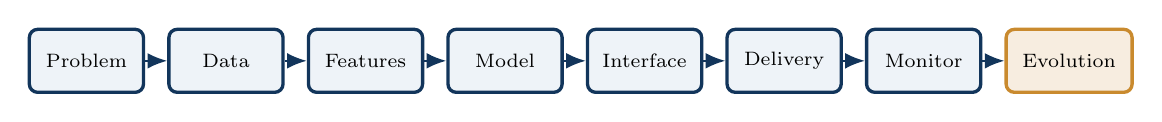
\begin{tikzpicture}[node distance=0.28cm]
  \node[flowbox, minimum width=1.45cm, minimum height=0.8cm] (problem) {\scriptsize Problem};
  \node[flowbox, minimum width=1.45cm, minimum height=0.8cm, right=of problem] (data) {\scriptsize Data};
  \node[flowbox, minimum width=1.45cm, minimum height=0.8cm, right=of data] (features) {\scriptsize Features};
  \node[flowbox, minimum width=1.45cm, minimum height=0.8cm, right=of features] (model) {\scriptsize Model};
  \node[flowbox, minimum width=1.45cm, minimum height=0.8cm, right=of model] (interface) {\scriptsize Interface};
  \node[flowbox, minimum width=1.45cm, minimum height=0.8cm, right=of interface] (delivery) {\scriptsize Delivery};
  \node[flowbox, minimum width=1.45cm, minimum height=0.8cm, right=of delivery] (monitor) {\scriptsize Monitor};
  \node[accentbox, minimum width=1.6cm, minimum height=0.8cm, right=of monitor] (evolution) {\scriptsize Evolution};
  \foreach \a/\b in {problem/data,data/features,features/model,model/interface,interface/delivery,delivery/monitor,monitor/evolution} {
    \draw[arrow] (\a) -- (\b);
  }
  \end{tikzpicture}

  \vspace{0.5em}
  \begin{block}{Today in the course}
  \textbf{Focus:} #1

  \textbf{Bridge:} #2
  \end{block}

  \begin{columns}[T]
  \column{0.48\textwidth}
  \begin{block}{Fraud case}
  {\footnotesize #3}
  \end{block}
  \column{0.48\textwidth}
  \begin{block}{Pasteurization case}
  {\footnotesize #4}
  \end{block}
  \end{columns}

  \vspace{0.3em}
  {\footnotesize \textbf{Course thread:} #5}
  \coursefooter
  \end{frame}
}

\newcommand{\classclosingframe}[4]{
  \begin{frame}{From This Class to the Next}
  \begin{block}{What stays with us}
  #1
  \end{block}

  \begin{columns}[T]
  \column{0.48\textwidth}
  \begin{block}{Project use}
  {\footnotesize #2}
  \end{block}
  \column{0.48\textwidth}
  \begin{block}{Next connection}
  {\footnotesize #3}
  \end{block}
  \end{columns}

  \vspace{0.3em}
  {\footnotesize \textbf{Course thread:} #4}
  \coursefooter
  \end{frame}
}

\tikzset{
  flowbox/.style={
    rounded corners=3pt,
    draw=courseblue,
    fill=courseice,
    very thick,
    minimum width=2.2cm,
    minimum height=0.9cm,
    align=center,
    font=\small
  },
  accentbox/.style={
    rounded corners=3pt,
    draw=coursegold,
    fill=coursegold!15,
    very thick,
    minimum width=2.2cm,
    minimum height=0.9cm,
    align=center,
    font=\small
  },
  arrow/.style={
    -{Latex[length=2.5mm,width=2mm]},
    thick,
    draw=courseblue
  }
}


\title{Class 14: Structured Data, Encoding, and Embeddings}
\author{\coursename}
\date{}

\begin{document}

\frame{\titlepage \coursefooter}

\begin{frame}{Agenda}
\begin{itemize}
\item From data type to data structure: structured, semi-structured, unstructured.
\item Where each structure shows up in this repository's real services.
\item Why raw values must be encoded before a model can use them.
\item One-hot, ordinal, target, and cyclic encoding.
\item Encoding versus embedding as two different compression strategies.
\item Dimensionality reduction (PCA) as feature extraction after encoding.
\end{itemize}
\coursefooter
\end{frame}

\begin{frame}{Learning goals}
\learninggoals{
\begin{itemize}
\item Classify a dataset as structured, semi-structured, or unstructured, and explain why the distinction matters.
\item Choose an encoding strategy that matches a variable's cardinality and meaning.
\item Explain the difference between a manually designed encoding and a learned embedding.
\item Understand PCA as one instance of a broader idea: compressing a representation once it is numeric.
\end{itemize}
}
\coursefooter
\end{frame}

\coursecontextframe
{Structured, semi-structured, and unstructured data, and the encoding and embedding theory that turns any of them into numbers.}
{Class 13 asked what kind of data we have. This class asks how it is organized, and how we turn it into the numeric representation every model actually consumes.}
{The fraud dataset is structured and already partly encoded: `V1`--`V28` are anonymized, PCA-derived numeric columns rather than raw transaction attributes.}
{The pasteurization service exchanges semi-structured JSON events over its streaming endpoint, even though the underlying sensor values are simple numbers.}
{This class supplies the representation layer that feature engineering (Class 15) and modeling (Class 16--17) both depend on.}

\begin{frame}{From data type to data structure}
\begin{itemize}
\item Class 13 asked whether data is tabular, time series, spectral, or image.
\item This class asks a orthogonal question: how organized is it, structured, semi-structured, or unstructured?
\item Any of the four data types from Class 13 can appear in any of these three organizational forms.
\item The organizational form determines how much encoding work is needed before a model can use the data at all.
\end{itemize}
\coursefooter
\end{frame}

\begin{frame}{Structured, semi-structured, and unstructured data}
\begin{tabularx}{\textwidth}{>{\bfseries}l X}
Structured & Fixed schema, fits directly into rows and columns: a CSV file or a SQL table. \\
Semi-structured & Has organization (keys, tags, nesting) but no fixed column schema: JSON logs, XML documents, API payloads. \\
Unstructured & No inherent schema at all: raw text, images, and audio waveforms. \\
\end{tabularx}
\coursefooter
\end{frame}

\begin{frame}{The taxonomy as a tree}
\centering
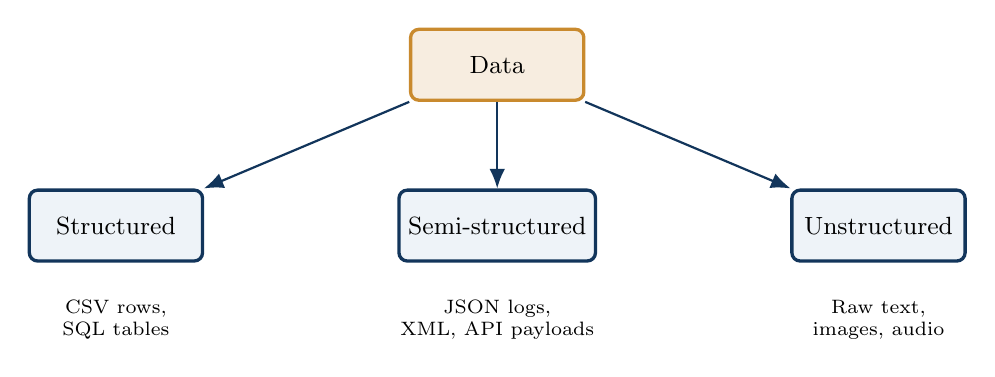
\begin{tikzpicture}[node distance=0.9cm and 0.6cm]
\node[accentbox] (root) {Data};
\node[flowbox, below left=1.1cm and 2.6cm of root] (s) {Structured};
\node[flowbox, below=1.1cm of root] (ss) {Semi-structured};
\node[flowbox, below right=1.1cm and 2.6cm of root] (u) {Unstructured};
\draw[arrow] (root) -- (s);
\draw[arrow] (root) -- (ss);
\draw[arrow] (root) -- (u);
\node[below=0.35cm of s, font=\scriptsize, align=center] {CSV rows,\\SQL tables};
\node[below=0.35cm of ss, font=\scriptsize, align=center] {JSON logs,\\XML, API payloads};
\node[below=0.35cm of u, font=\scriptsize, align=center] {Raw text,\\images, audio};
\end{tikzpicture}
\coursefooter
\end{frame}

\begin{frame}{Semi-structured data in this course's own services}
\begin{itemize}
\item It is tempting to think of this course as purely tabular, but two real services already speak semi-structured data.
\item A Flask endpoint receiving `request.get_json(force=True)` is accepting a semi-structured payload before it is ever turned into a feature array.
\item The pasteurization streaming endpoint emits one semi-structured JSON event per second, not a table.
\item Both are converted into structured, tabular inputs before a model touches them.
\end{itemize}
\coursefooter
\end{frame}

\begin{frame}[fragile]{Semi-structured example: a streaming JSON event}
\begin{lstlisting}[style=coursepython]
def generate():
    for _, row in df.iterrows():
        data = row.to_dict()
        yield f"data: {json.dumps(data)}\n\n"
        time.sleep(STREAM_DT)
\end{lstlisting}
\begin{itemize}
\item From `pasteurization/serving.py`: each streamed event is a small, self-describing JSON object with named keys.
\item Nothing forces every event to have the same keys, which is exactly what distinguishes semi-structured data from a rigid table.
\end{itemize}
\coursefooter
\end{frame}

\begin{frame}{Unstructured data}
\begin{itemize}
\item Raw text, images, and audio carry no built-in fields or schema; meaning has to be extracted, not read off a column name.
\item Unstructured data almost always requires a learned representation (an embedding) rather than a small set of hand-designed columns.
\item None of this repository's two running cases uses unstructured data directly, but production fraud and process-monitoring systems often also ingest free-text notes, images, or logs alongside their tabular core.
\item The encoding and embedding ideas in this class scale from ``one categorical column'' up to ``an entire document or image''.
\end{itemize}
\coursefooter
\end{frame}

\begin{frame}{Why encoding exists}
\begin{itemize}
\item Models compute with numbers; most raw variables (categories, labels, identifiers) are not numbers.
\item Encoding is the deliberate, documented choice of how a symbolic value becomes a numeric one.
\item A bad encoding can inject a false sense of order, leak information, or blow up dimensionality.
\item The right choice depends on cardinality (how many distinct values) and semantics (does order mean anything).
\end{itemize}
\coursefooter
\end{frame}

\begin{frame}{Encoding choices}
\begin{tabularx}{\textwidth}{>{\bfseries}l X}
One-hot encoding & Good for low-cardinality categories with no natural order. \\
Ordinal encoding & Use only when order is real and meaningful. \\
Target encoding & Useful for high-cardinality categories, but must control leakage. \\
Cyclic encoding & Useful for hour-of-day, day-of-week, and other seasonal variables. \\
\end{tabularx}
\coursefooter
\end{frame}

\begin{frame}[fragile]{Encoding example: structured pipeline with one-hot encoding}
\begin{lstlisting}[style=coursepython]
categorical_features = ["pclass", "sex", "embarked", "title"]

categorical_transformer = Pipeline(steps=[
    ("encoder", OneHotEncoder(handle_unknown="ignore"))
])

preprocessor = ColumnTransformer(
    transformers=[
        ("num", numeric_transformer, numeric_features),
        ("cat", categorical_transformer, categorical_features)
    ]
)
\end{lstlisting}
\begin{itemize}
\item From `notebooks/Class4_DataEngineering.ipynb`: encoding is expressed as an explicit, reusable pipeline step, not an ad hoc conversion.
\item `handle_unknown="ignore"` is itself an encoding decision: what happens when a category appears at inference time that training never saw.
\end{itemize}
\coursefooter
\end{frame}

\begin{frame}{Encoding versus embedding}
\begin{tabularx}{\textwidth}{>{\bfseries}l X}
Encoding & A manually designed, usually sparse mapping from symbols to numbers (one-hot, ordinal, target). \\
Embedding & A learned, dense, lower-dimensional vector that a model fits to place similar items close together. \\
\end{tabularx}
\begin{itemize}
\item Encodings are interpretable by construction; embeddings are compact but usually opaque.
\item Text embeddings (word2vec-style) and learned image features play the same role for unstructured data that one-hot encoding plays for a categorical column.
\item The choice is not ideological: high-cardinality categories and unstructured data push naturally toward embeddings.
\end{itemize}
\coursefooter
\end{frame}

\begin{frame}{Feature extraction: compressing after encoding}
\begin{itemize}
\item Once every variable is numeric, we can ask a second, different question: can we compress this representation without losing what matters?
\item Feature extraction transforms an already-numeric representation into a smaller one, rather than deciding how to encode a single symbol.
\item PCA is the classical linear technique for structured, tabular data.
\item The same idea has data-type-specific analogues: the Fourier transform or MFCC framing for signals, and learned convolutional or embedding features for images and text.
\end{itemize}
\coursefooter
\end{frame}

\begin{frame}{PCA intuition}
PCA rotates the original feature space to new orthogonal axes called principal components, ordered by the amount of variance they explain.
\vspace{0.5em}
\begin{itemize}
\item The first component captures the largest possible variance; later components capture what is left, subject to orthogonality.
\item Keeping only the leading components compresses the representation while trying to preserve most of the structure.
\item PCA must be fit only on training data, then applied identically at inference time.
\end{itemize}
\coursefooter
\end{frame}

\begin{frame}[fragile]{Feature extraction example: PCA after encoding}
\begin{lstlisting}[style=coursepython]
pca_pipeline = Pipeline(steps=[
    ("preprocessor", preprocessor),
    ("pca", PCA(n_components=3)),
    ("classifier", LogisticRegression(max_iter=100))
])

pca_pipeline.fit(X_train, y_train)
y_pred_pca = pca_pipeline.predict(X_test)
\end{lstlisting}
\begin{itemize}
\item From `notebooks/Class4_DataEngineering.ipynb`: PCA is inserted as one more pipeline stage, right after encoding and scaling.
\item This is the same ordering principle as the taxonomy in this class: encode first, then decide whether to compress.
\end{itemize}
\coursefooter
\end{frame}

\begin{frame}{PCA projection with feature directions}
\centering
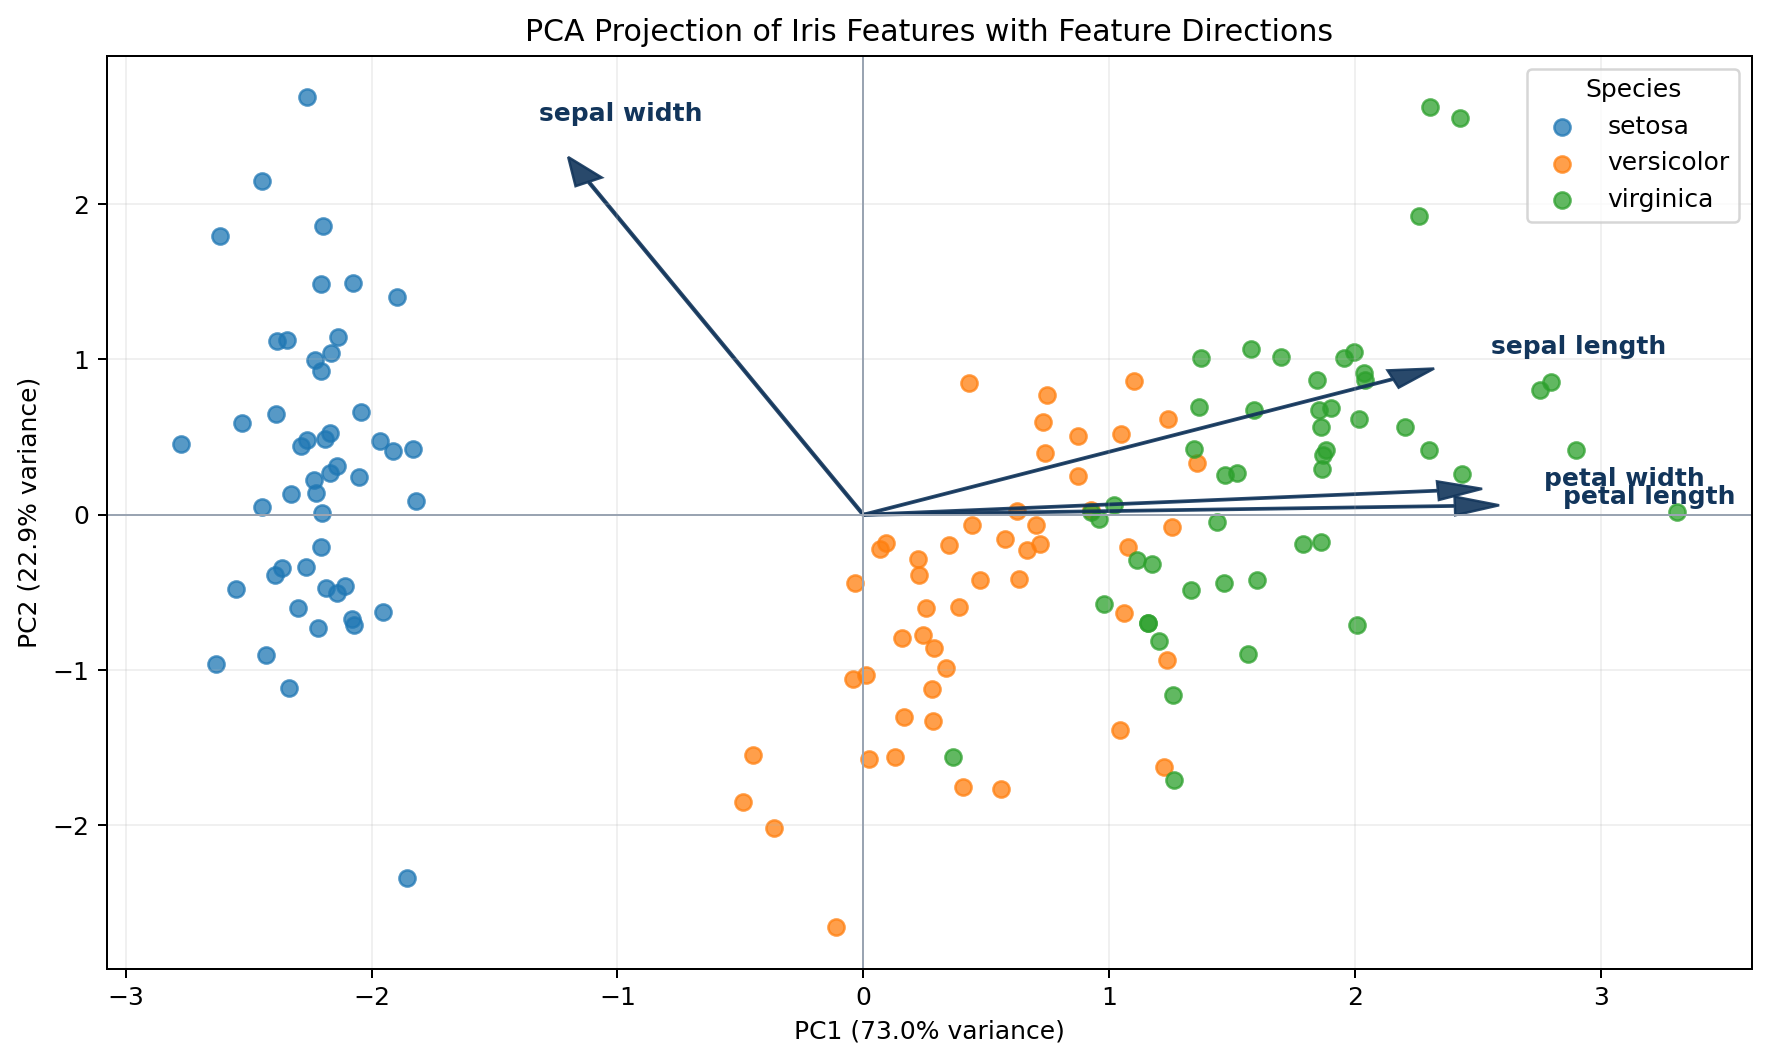
\includegraphics[height=0.7\textheight]{images/class03_pca_yellowbrick_style.png}

{\scriptsize Recreated from `notebooks/Class3_PCA.ipynb`: once features are numeric, PCA re-expresses them along the directions of largest variance.}
\coursefooter
\end{frame}

\begin{frame}{Analogues across data types, and the fraud case}
\begin{tabularx}{\textwidth}{>{\bfseries}l X}
Tabular & PCA on encoded, scaled columns. \\
Signal & Fourier transform or MFCC framing before modeling. \\
Image / text & Learned convolutional or embedding features. \\
\end{tabularx}
\vspace{0.4em}
\begin{block}{Fraud example}
The fraud dataset already ships with PCA-derived variables `V1`--`V28`. The encoding and extraction steps happened before the data ever reached this course; the original attributes are permanently hidden.
\end{block}
\coursefooter
\end{frame}

\begin{frame}{Repository connections}
\repoactivity{
\begin{itemize}
\item `notebooks/Class4_DataEngineering.ipynb` shows encoding (`OneHotEncoder`) and extraction (`PCA`) as consecutive pipeline stages.
\item `pasteurization/serving.py` produces the semi-structured JSON stream that a later stage turns into structured features.
\item The fraud dataset's `V1`--`V28` columns are a real example of encoding and extraction decisions made upstream, outside our control.
\end{itemize}
}
\coursefooter
\end{frame}

\begin{frame}{Discussion prompt}
\begin{block}{Question}
If the fraud dataset's `V1`--`V28` are PCA components, what did we lose by never seeing the original raw attributes?
\end{block}
\begin{itemize}
\item This connects representation choices back to interpretability, a theme that returns in Class 17's decision-making discussion.
\end{itemize}
\coursefooter
\end{frame}

\begin{frame}{Papers and materials}
\readinglist{
\href{https://www.oreilly.com/library/view/feature-engineering-for/9781491953235/}{Zheng and Casari, Feature Engineering for Machine Learning};\
\href{https://scikit-learn.org/stable/modules/generated/sklearn.compose.ColumnTransformer.html}{ColumnTransformer};\
\href{https://scikit-learn.org/stable/modules/decomposition.html\#pca}{scikit-learn PCA guide};\
\href{https://link.springer.com/book/10.1007/b98835}{Jolliffe, Principal Component Analysis};\
\href{https://www.oreilly.com/library/view/designing-machine-learning/9781098107956/}{Chip Huyen, Designing Machine Learning Systems}.
}
\coursefooter
\end{frame}

\classclosingframe
{\begin{itemize}
\item Structured, semi-structured, and unstructured data need increasingly deliberate representation work before modeling.
\item Encoding is a manual, interpretable mapping; embeddings are learned, dense, and compact.
\item Dimensionality reduction such as PCA is feature extraction: compression applied after encoding, not a replacement for it.
\end{itemize}}
{Project teams should now be able to name, for every raw input, whether it needs encoding, an embedding, or both, and whether extraction is worth the interpretability cost.}
{Class 15 uses this numeric representation to clean, curate, select, and construct the actual features a model will train on.}
{Data type (Class 13) and representation (Class 14) together set up feature engineering (Class 15) as a design activity, not guesswork.}

\end{document}
